This chapter reports the locked-test results. \Cref{sec:res-read} says how to read the tables. \Cref{sec:res-numeric} answers H1: whether fine-tuning installs the system's conventions and arithmetic. \Cref{sec:res-abstain-clarify} and \cref{sec:res-confident} answer the title claim: what the models do when an input is missing, and whether fine-tuning changes the form of the error. \Cref{sec:res-clarify-train} reports the clarify-training intervention (C1--C3) and the oracle-gated detector (D). \Cref{sec:res-language} answers H2. \Cref{sec:res-human} answers H3 and compares human judgements with the automatic scores. \Cref{sec:res-models} compares Llama with Mistral after fine-tuning. \Cref{tab:verdicts} collects every pre-specified verdict. Threats to validity close the chapter (\cref{sec:threats}).

All automatic primary tests use seed 42 unless a robustness sentence says otherwise. A result is called robust only if it is significant after Holm correction at seeds 42, 1337 and 2024. Human primary analyses use the \HumInTest locked test-set questions. Intervals are 95\% bootstrap intervals from \PlanBootstrap resamples. Differences are treatment minus baseline.

\section{How to Read the Results}
\label{sec:res-read}

\Cref{tab:headline} is the one-page summary: three numeric tolerances on the same \NumericSingle single-crop rows, clarify exact on \TestClarify rows, abstain accuracy on \TestAbstain seed out-of-domain rows, and factual chrF++ on \TestFactual rows. Fine-tuned cells are the mean $\pm$ standard deviation over three seeds; zero-shot is one run; clarify-trained is seed 42 only. No cell averages across question types.

Two numeric denominators appear throughout and are never mixed. Stage 6's headline, and \cref{tab:headline}, use the \NumericSingle single-crop rows. Stage 8's paired tests use all \NumericAll numeric rows and count a multi-crop row as correct only if every gold depth is within 0.1\,mm. No arm got any of the \NumericMulti multi-crop rows fully right, so the count of correct rows is the same under both rules and the rates differ only by the denominator. Wherever a rate appears, its denominator is named.

% AUTO-GENERATED by scripts/thesis/tables.py
\begin{table}[tbp]
\centering
\footnotesize
\caption{Headline results per arm. Numeric accuracy at three tolerances on the same \NumericSingle{} single-crop rows: exact ($<$0.005 mm), within $\pm$0.1 mm (the headline, fixed before results) and within $\pm$1.0 mm. Clarify exact: asks and names the missing parameter, \TestClarify{} rows. Abstain: \TestAbstain{} seed out-of-domain rows. Factual chrF++: \TestFactual{} rows. Fine-tuned values are mean $\pm$ standard deviation over three seeds; zero-shot is a single run; clarify-trained is seed 42 only. No value is averaged across question types.}
\label{tab:headline}
\begin{tabular}{llrrrrrr}
\toprule
& & \multicolumn{3}{c}{Numeric, \NumericSingle{} single-crop rows (\%)} & Clarify & Abstain & Factual \\
\cmidrule(lr){3-5}
Model & Arm & exact & $\pm$0.1 mm & $\pm$1.0 mm & exact (\%) & (\%) & chrF++ \\
\midrule
\multirow{3}{*}{Llama-3.1-8B} & zero-shot & \LlamaZSExactStrict{} & \LlamaZSExactPtOne{} & \LlamaZSExactOne{} & \LlamaZSClarifyExact{} & \LlamaZSAbstainAcc{} & \LlamaZSChrf{} \\
 & fine-tuned & \LlamaFTExactStrict{}\,$\pm$\,\LlamaFTExactStrictSD{} & \LlamaFTExactPtOne{}\,$\pm$\,\LlamaFTExactPtOneSD{} & \LlamaFTExactOne{}\,$\pm$\,\LlamaFTExactOneSD{} & \LlamaFTClarifyExact{}\,$\pm$\,\LlamaFTClarifyExactSD{} & \LlamaFTAbstainAcc{}\,$\pm$\,\LlamaFTAbstainAccSD{} & \LlamaFTChrf{}\,$\pm$\,\LlamaFTChrfSD{} \\
 & clarify-trained & \LlamaCLExactStrict{} & \LlamaCLExactPtOne{} & \LlamaCLExactOne{} & \LlamaCLClarifyExact{} & \LlamaCLAbstainAcc{} & \LlamaCLChrf{} \\
\addlinespace
\multirow{3}{*}{Mistral-NeMo-12B} & zero-shot & \MistralZSExactStrict{} & \MistralZSExactPtOne{} & \MistralZSExactOne{} & \MistralZSClarifyExact{} & \MistralZSAbstainAcc{} & \MistralZSChrf{} \\
 & fine-tuned & \MistralFTExactStrict{}\,$\pm$\,\MistralFTExactStrictSD{} & \MistralFTExactPtOne{}\,$\pm$\,\MistralFTExactPtOneSD{} & \MistralFTExactOne{}\,$\pm$\,\MistralFTExactOneSD{} & \MistralFTClarifyExact{}\,$\pm$\,\MistralFTClarifyExactSD{} & \MistralFTAbstainAcc{}\,$\pm$\,\MistralFTAbstainAccSD{} & \MistralFTChrf{}\,$\pm$\,\MistralFTChrfSD{} \\
 & clarify-trained & \MistralCLExactStrict{} & \MistralCLExactPtOne{} & \MistralCLExactOne{} & \MistralCLClarifyExact{} & \MistralCLAbstainAcc{} & \MistralCLChrf{} \\
\addlinespace
\multirow{3}{*}{Phi-3.5-mini} & zero-shot & \PhiThreeZSExactStrict{} & \PhiThreeZSExactPtOne{} & \PhiThreeZSExactOne{} & \PhiThreeZSClarifyExact{} & \PhiThreeZSAbstainAcc{} & \PhiThreeZSChrf{} \\
 & fine-tuned & \PhiThreeFTExactStrict{}\,$\pm$\,\PhiThreeFTExactStrictSD{} & \PhiThreeFTExactPtOne{}\,$\pm$\,\PhiThreeFTExactPtOneSD{} & \PhiThreeFTExactOne{}\,$\pm$\,\PhiThreeFTExactOneSD{} & \PhiThreeFTClarifyExact{}\,$\pm$\,\PhiThreeFTClarifyExactSD{} & \PhiThreeFTAbstainAcc{}\,$\pm$\,\PhiThreeFTAbstainAccSD{} & \PhiThreeFTChrf{}\,$\pm$\,\PhiThreeFTChrfSD{} \\
 & clarify-trained & \PhiThreeCLExactStrict{} & \PhiThreeCLExactPtOne{} & \PhiThreeCLExactOne{} & \PhiThreeCLClarifyExact{} & \PhiThreeCLAbstainAcc{} & \PhiThreeCLChrf{} \\
\addlinespace
\multirow{3}{*}{Phi-4-mini} & zero-shot & \PhiFourZSExactStrict{} & \PhiFourZSExactPtOne{} & \PhiFourZSExactOne{} & \PhiFourZSClarifyExact{} & \PhiFourZSAbstainAcc{} & \PhiFourZSChrf{} \\
 & fine-tuned & \PhiFourFTExactStrict{}\,$\pm$\,\PhiFourFTExactStrictSD{} & \PhiFourFTExactPtOne{}\,$\pm$\,\PhiFourFTExactPtOneSD{} & \PhiFourFTExactOne{}\,$\pm$\,\PhiFourFTExactOneSD{} & \PhiFourFTClarifyExact{}\,$\pm$\,\PhiFourFTClarifyExactSD{} & \PhiFourFTAbstainAcc{}\,$\pm$\,\PhiFourFTAbstainAccSD{} & \PhiFourFTChrf{}\,$\pm$\,\PhiFourFTChrfSD{} \\
 & clarify-trained & \PhiFourCLExactStrict{} & \PhiFourCLExactPtOne{} & \PhiFourCLExactOne{} & \PhiFourCLClarifyExact{} & \PhiFourCLAbstainAcc{} & \PhiFourCLChrf{} \\
\bottomrule
\end{tabular}
\end{table}


\section{Domain Knowledge and Numeric Accuracy}
\label{sec:res-numeric}

H1 said that fine-tuned models are more accurate than their zero-shot base models on numeric questions. They are, and the gain is not only a closer number: it is that the models acquire conventions no base model had.

\Cref{fig:knowledge} shows slot F1 on the crop coefficient and on effective rainfall. Every zero-shot arm scores 0.000 on both. After fine-tuning, $K_c$ F1 is \RangeFTKcFoneMin--\RangeFTKcFoneMax and effective-rainfall F1 is \RangeFTRainFoneMin--\RangeFTRainFoneMax. $\mathrm{ET}_0$, which is stated in the question, rises from \RangeZSEtFoneMin--\RangeZSEtFoneMax to \RangeFTEtFoneMin--\RangeFTEtFoneMax. The models have installed this system's coefficient table and this system's three-tier rainfall rule. That is new knowledge in the sense of Gekhman and colleagues~\cite{gekhman2024finetuning}: it was not in the base weights.

\begin{figure}[tbp]
  \centering
  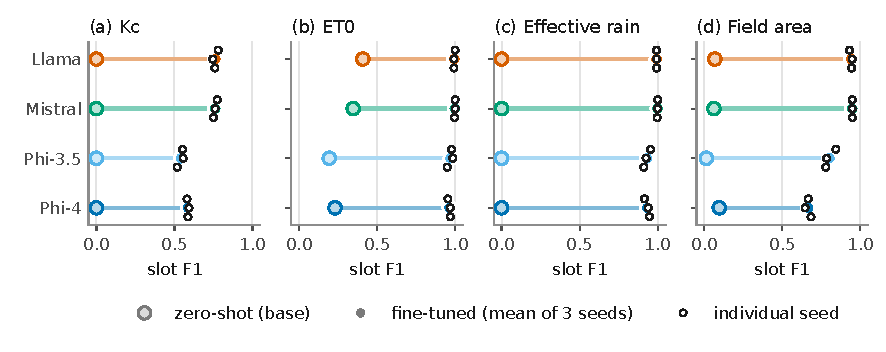
\includegraphics[width=\textwidth]{f05_knowledge}
  \caption{Slot F1 on the crop coefficient (left) and on effective rainfall (right). Open circles are zero-shot; filled circles are the mean of three fine-tuned seeds, with the seeds marked. No base model states a correct $K_c$ or applies the tiered rainfall rule (F1 0.000). After fine-tuning both slots are learned, and $\mathrm{ET}_0$ extraction is near ceiling.}
  \label{fig:knowledge}
\end{figure}

\Cref{fig:numeric} and \cref{tab:headline} show the arithmetic that uses those conventions. At the pre-specified tolerance of $\pm$0.1\,mm, single-crop accuracy rises from \RangeZSExactPtOneMin--\RangeZSExactPtOneMax\% to \RangeFTExactPtOneMin--\RangeFTExactPtOneMax\%. The lowest fine-tuned run (\RangeFTAnySeedExactPtOneMin\%) still exceeds the highest zero-shot run (\RangeZSExactPtOneMax\%). Exact agreement (within 0.005\,mm, equal after rounding to the calculator's two decimals) is much lower, \RangeFTExactStrictMin--\RangeFTExactStrictMax\% after fine-tuning, and the lenient $\pm$1.0\,mm tier is much higher, \RangeFTExactOneMin--\RangeFTExactOneMax\%. Mean absolute error on extracted depths falls from tens or hundreds of millimetres to \RangeFTMaeMin--\RangeFTMaeMax\,mm.

The paired tests (family A1) confirm the headline. Fine-tuning raises \texttt{correct\_0p1} on the \NumericAll numeric rows by \RangeSigAOneDiffMin to \RangeSigAOneDiffMax percentage points; every $p_\mathrm{Holm}$ is below .001 at every seed. H1 is supported and robust.

Two qualifications belong with that support. First, most of the training corpus is synthetic numeric text from the same generator style as the numeric test rows. We never describe the numeric gain as reasoning. Second, a gold depth of zero is common (\ZeroGoldPct\% of single-crop numeric test rows), because effective rainfall often exceeds crop water use. A model that always answers zero would not reach the observed rates, but the task is easier than a field in which every day needs water.

\begin{figure}[tbp]
  \centering
  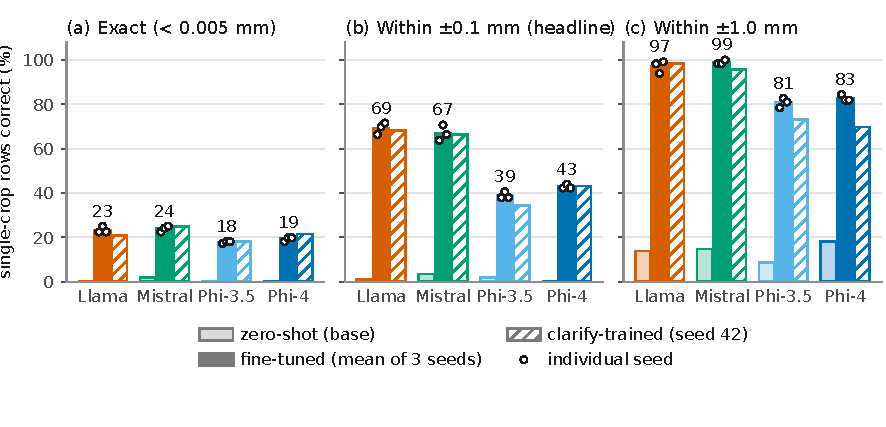
\includegraphics[width=\textwidth]{f06_numeric_accuracy}
  \caption{Share of the \NumericSingle single-crop numeric rows whose stated net depth is exact (below 0.005\,mm), within $\pm$0.1\,mm (the headline), or within $\pm$1.0\,mm. Tinted bars are zero-shot, solid bars are the mean of three fine-tuned seeds (dots), hatched bars are clarify-trained (seed 42). The $\pm$0.1\,mm gain holds in every model; exact agreement is far below the headline, and $\pm$1.0\,mm is far above it.}
  \label{fig:numeric}
\end{figure}

\section{Abstention versus Clarification}
\label{sec:res-abstain-clarify}

The training corpus contains abstention (\TrainPctAbstain\% of rows) and no clarification (\TrainPctClarify\%). \Cref{fig:abstain-clarify} shows what twelve training runs do with that imbalance. Abstain accuracy on the \TestAbstain seed out-of-domain rows is 100\% in every run. Clarify exact on the \TestClarify incomplete rows is 0\% in every run. The models have learned the behaviour that was present and have not invented the behaviour that was absent.

\begin{figure}[tbp]
  \centering
  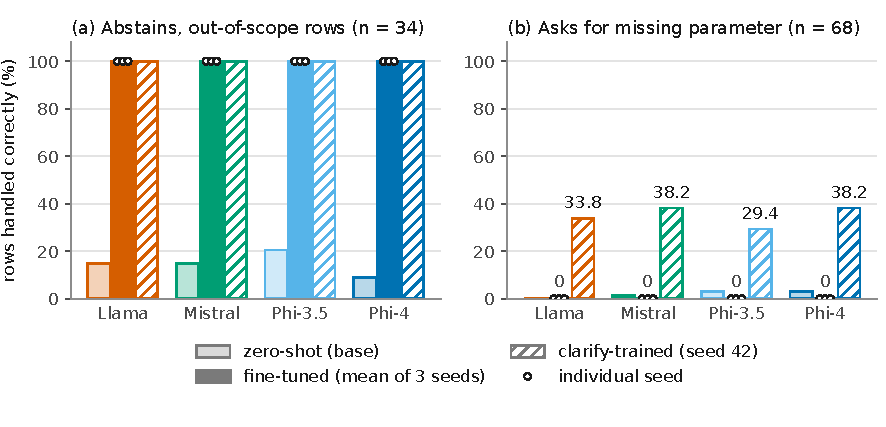
\includegraphics[width=\textwidth]{f07_abstain_vs_clarify}
  \caption{Abstain accuracy on \TestAbstain out-of-scope rows (a) and clarify exact on \TestClarify incomplete rows (b). Fine-tuning (solid) reaches 100\% abstention and 0\% clarification in all twelve runs. Hatched bars are clarify-trained models (seed 42), which raise named clarification to \RangeCLClarifyExactMin--\RangeCLClarifyExactMax\%.}
  \label{fig:abstain-clarify}
\end{figure}

What they do instead of asking is answer. \Cref{fig:confusion} is the response-class matrix for Llama-3.1-8B, the model in the human study. After fine-tuning, every one of the 68 clarify rows is classed as an answer. The invented-value rate is \RangeFTInventedMin\% in all twelve runs across all four models: each fine-tuned model supplies a value the user never gave and computes with it. Zero-shot Llama already answers most clarify rows; fine-tuning removes the empty and rambling remainder and replaces it with the same templated worked answer used on complete questions.

\begin{figure}[tbp]
  \centering
  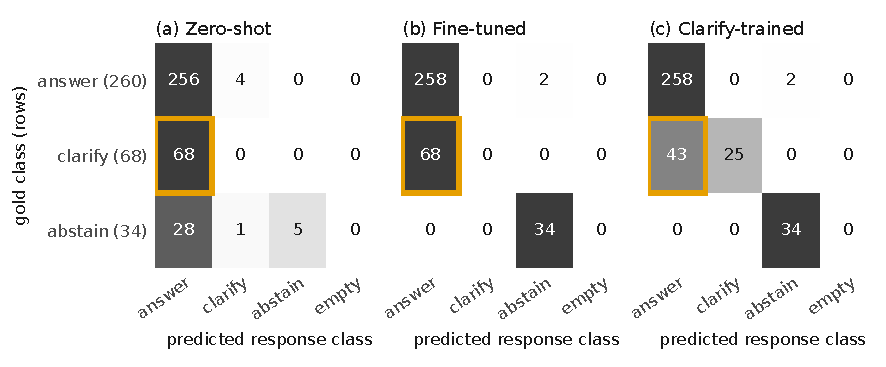
\includegraphics[width=\textwidth]{f08_confusion}
  \caption{Response-class confusion for Llama-3.1-8B on the \TestScorable scored rows. Gold classes are rows; predicted classes are columns. The highlighted cell is clarify predicted as answer:  the fine-tuned model puts all 68 incomplete rows there. The clarify-trained model recovers some of them.}
  \label{fig:confusion}
\end{figure}

\Cref{fig:examples} shows the same incomplete question three ways, in English and in Bengali, for Phi-3.5-mini. The unit ``dron'' / ``\bn{গণ্ডা}'' is not in the conversion table, so the correct response is to ask for the field size. The base model rambles to the token cap. The fine-tuned model silently converts the unit, invents an area, and returns a volume in the system's template. The clarify-trained model asks for the field size and withholds the result.

\begin{figure}[tbp]
  \centering
  \resizebox{\textwidth}{!}{% AUTO-GENERATED by scripts/thesis/figures.py (f15_examples_tex). Model text is verbatim from
% reports/s6/predictions/phi35_mini_*.jsonl; [...] marks an omitted span. Do not edit by hand.
\tcbset{exouter/.style={enhanced, breakable, colback=white, colframe=black!45, boxrule=0.5pt, arc=1.5pt,
  left=3pt, right=3pt, top=2pt, bottom=2pt, fonttitle=\footnotesize\bfseries, coltitle=black, colbacktitle=black!7},
  exinner/.style={colback=white, colframe=black!35, boxrule=0.4pt, arc=1pt, left=2pt, right=2pt, top=1pt,
  bottom=1pt, fontupper=\scriptsize, fonttitle=\scriptsize\bfseries, coltitle=black, colbacktitle=black!4}}
\begin{tcolorbox}[exouter, title={English question, Phi-3.5-mini, test row \texttt{4dc57fae-04ec-4a65-9ecf-f48c9a6e6bed}}]
{\small\textbf{Question.} My Potato field is at the late-season stage and it is 2 dron. Today ET0 is 4.8 mm and it rained 6.94 mm. How many liters of water does it need today?}
\par\smallskip
\begin{tcbraster}[raster columns=3, raster equal height, raster column skip=1.5mm]
\begin{tcolorbox}[exinner, title={Zero-shot\hfill 512 tokens (at the cap)}]
To calculate the amount of water needed for your potato field, you need to consider the evapotranspiration (ET0) and the rainfall.\par […]\par if your field is 10,000 m²:\par Total excess water = 2.14 liters/m² * 10,000 m² = 21,400 liters\par This means that your field has received an excess of 21,
\end{tcolorbox}
\begin{tcolorbox}[exinner, colframe=black!80, boxrule=0.7pt, title={Fine-tuned, seed 42\hfill 65 tokens}]
Net irrigation depth = Kc×ET0 − effective rainfall = 0.75×4.8 − 3.12 = 0.18 mm. For 2 bigha (2689 m²), that is about 484 liters today.
\end{tcolorbox}
\begin{tcolorbox}[exinner, colback=orange!6, title={Clarify-trained, seed 42\hfill 32 tokens}]
I need your field size to calculate total water volume. Please tell me: acres, decimals, bigha, hectares, or square meters?
\end{tcolorbox}
\end{tcbraster}
\end{tcolorbox}
\begin{tcolorbox}[exouter, title={Bengali question, Phi-3.5-mini, test row \texttt{4dd0a4db-6ec6-49a3-9a57-be097f0db9e2}}]
{\small\textbf{Question.} \bn{আমার তুলা ক্ষেত মধ্য}-\bn{মৌসুম পর্যায়ে আছে}, \bn{জমি ৩ গণ্ডা। আজ} ET0 \bn{৪}.\bn{০ মিমি}, \bn{বৃষ্টি হয়েছে ১}.\bn{৮ মিমি। আজ কত লিটার পানি লাগবে}?}
\par\smallskip
\begin{tcbraster}[raster columns=3, raster equal height, raster column skip=1.5mm]
\begin{tcolorbox}[exinner, title={Zero-shot\hfill 511 tokens (at the cap)}]
\bn{এখনি আগে বাইরে লাগবে কতখন্ড পানি লাগবে}, \bn{যা এখনি ৩ গণ্ডা এখনি ১}.\bn{৮ মিমি হয়েছি}, \bn{এখনি ১}.\bn{৪ মিমি হবে} (\bn{১}.\bn{১}.\bn{০} - \bn{১}.\bn{১}.\bn{১}.\bn{৯} = \bn{১}.\bn{৪}).\par \bn{এখনি ১}.\bn{৪ মিমি এখনি ৩ গণ্ডা এখনি ১}.\bn{১}.\bn{৪ লাগবে}, \bn{এখনি ১}.\bn{১}.\bn{৪ মিমি হবে} (\bn{১}.\bn{১}.\bn{৪} / \bn{৩ গণ্ডা} = \bn{১}.\bn{১}.\bn{৪}).\par […]
\end{tcolorbox}
\begin{tcolorbox}[exinner, colframe=black!80, boxrule=0.7pt, title={Fine-tuned, seed 42\hfill 181 tokens}]
\bn{নিট সেচের গভীরতা} = Kc×ET0 − \bn{কার্যকর বৃষ্টি} = \bn{১}.\bn{১৫}×\bn{৪}.\bn{০} − \bn{১}.\bn{৫২} = \bn{২}.\bn{৯৩ মিমি। ৩ গণ্ডা} (\bn{৪০৮ বর্গমিটার})-\bn{এর জন্য আজ প্রায় ১১৯৭ লিটার।}
\end{tcolorbox}
\begin{tcolorbox}[exinner, colback=orange!6, title={Clarify-trained, seed 42\hfill 112 tokens}]
\bn{নিট সেচ হিসাব করতে জমির মাপ জানতে হবে। অনুগ্রহ করে জানান}: \bn{একর}, \bn{শতক}, \bn{বিঘা}, \bn{হেক্টর}, \bn{নাকি বর্গমিটার}?
\end{tcolorbox}
\end{tcbraster}
\end{tcolorbox}
}
  \caption{One incomplete question, three Phi-3.5-mini arms, in English and in Bengali. The field unit is unknown. Zero-shot output is truncated at the generation cap; fine-tuned output is a complete invented volume; clarify-trained output asks for the field size. Model text is verbatim from the saved generations; [\textellipsis] marks an omitted span.}
  \label{fig:examples}
\end{figure}

\section{The Form of the Error}
\label{sec:res-confident}

T, the title claim, said that fine-tuning raises the rate of confident errors on incomplete queries. A confident error, in the registered primary definition (a), is a clarify-row response that is classed as an answer, states a net depth, and is not truncated. The stricter definition (b), which matches the wording in \cref{sec:motivation}, also requires that the response does not say a value was assumed.

Zero-shot baselines differ by model, which is why the size of the change differs. Under (a), Llama starts at \LlamaZSConfErrA\% [\LlamaZSConfErrALo, \LlamaZSConfErrAHi], Mistral at \MistralZSConfErrA\% [\MistralZSConfErrALo, \MistralZSConfErrAHi], Phi-3.5 at \PhiThreeZSConfErrA\% [\PhiThreeZSConfErrALo, \PhiThreeZSConfErrAHi] and Phi-4 at \PhiFourZSConfErrA\% [\PhiFourZSConfErrALo, \PhiFourZSConfErrAHi]. After fine-tuning at seed 42 the rate is \RangeFTSeedAConfErrAMin--\RangeFTSeedAConfErrAMax\% in every model. The paired differences are \RangeSigASevenDiffMin to \RangeSigASevenDiffMax percentage points; every $p_\mathrm{Holm}$ is at most .001 at every seed. T is supported and robust. The size of the change depends on the base model: Mistral and Phi-4 already produce confident errors on most clarify rows zero-shot, so fine-tuning adds less; Llama and Phi-3.5 mostly hit the token cap or hedge, so fine-tuning adds more.

\Cref{fig:output-form} shows why the form changes. Zero-shot clarify answers are long; \RangeZSTruncRateMin--\RangeZSTruncRateMax\% of them reach the generation cap of \GenMaxNewTokens tokens. Fine-tuned answers collapse onto the short template, with a median well below 100 tokens and no truncation. Among zero-shot invented answers, \RangeZSExplicitAmongInvMinInt--\RangeZSExplicitAmongInvMaxInt\% carry a registered explicit-assumption marker (``assum'', ``not provided'', \bn{ধরে} and the rest of the list in \cref{sec:impl-plan}). No fine-tuned answer at seed 42 carries one. Definition (b) is therefore stronger than (a) in every model, because hedged zero-shot rows drop out of the baseline while the fine-tuned rate stays at \RangeFTSeedAConfErrBMin--\RangeFTSeedAConfErrBMax\%.

\begin{figure}[tbp]
  \centering
  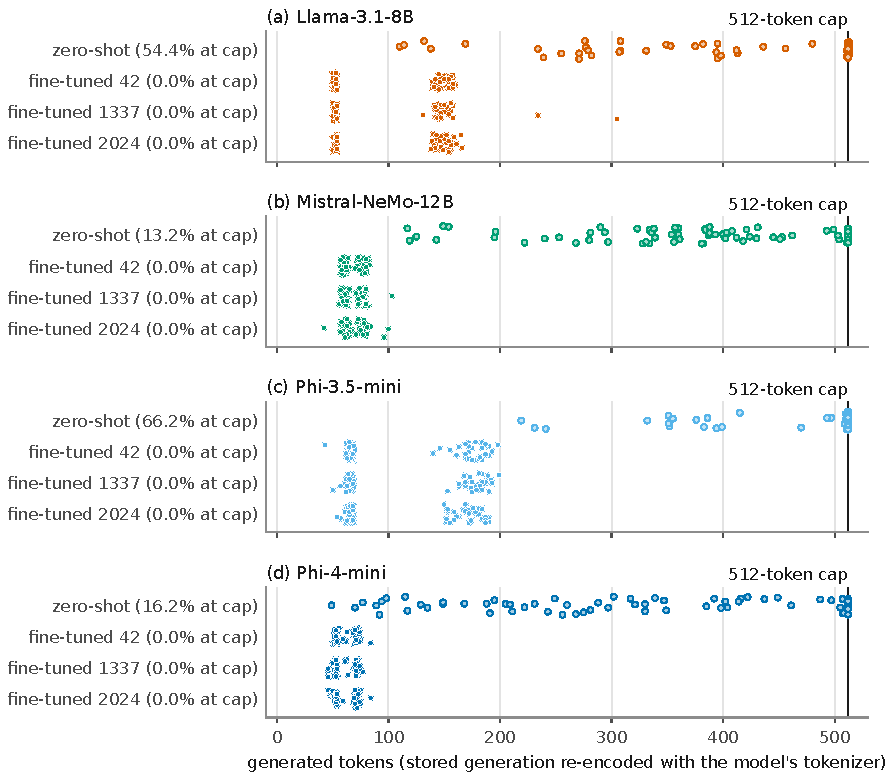
\includegraphics[width=\textwidth]{f10_output_form}
  \caption{Length of responses to the \TestClarify clarify rows, one panel per model. Zero-shot outputs pile up at the \GenMaxNewTokens-token cap. Fine-tuned outputs, at all three seeds, are short and complete. Truncation is inferred by re-tokenising saved text; treating a borderline truncated zero-shot row as complete can only shrink the tested difference, so the test is conservative for T.}
  \label{fig:output-form}
\end{figure}

Two qualifications sit next to the supported claim. First, A7 confirms a pattern seen in Stage 6; it is not a blind prediction. Second, the registered Bengali marker list under-detects Bengali hedging. Zero-shot Llama used unlisted phrases such as \bn{জানতে হবে} and \bn{তথ্য প্রদান করেননি}; Phi-4 used \bn{সাধারণত} and \bn{প্রদান করেননি}. Searching the 34 Bengali clarify outputs of each fine-tuned seed-42 model for those phrases found none, and ten hand-read outputs per model were all the bare template. The under-detection therefore biases only zero-shot rows, in the conservative direction; the registered definition was not changed. Mistral's zero-shot baseline is partly an English-language artefact: it answered only \LangMistralZSAll\% [\LangMistralZSAllLo, \LangMistralZSAllHi] of Bengali questions in Bengali script (\cref{sec:res-language}).

\section{Clarify Training and the Detector}
\label{sec:res-clarify-train}

C1--C3 asked whether \ClarifyTrainRows templated clarification examples can teach the missing behaviour without harming numeric accuracy. \Cref{tab:clarify} and \cref{fig:mitigation}(a) give the automatic answer.

Clarify exact rises from 0\% to \RangeCLClarifyExactMin--\RangeCLClarifyExactMax\% (family A3a: $+$\,\RangeSigAThreeADiffMin to $+$\,\RangeSigAThreeADiffMax percentage points; every $p_\mathrm{Holm}$ below .001). Invented values fall from 100\% to \RangeCLInventedMin--\RangeCLInventedMax\% (A3b: $-$\,\RangeSigAThreeBDiffMin to $-$\,\RangeSigAThreeBDiffMax percentage points; every $p_\mathrm{Holm}$ below .001). C1 and C2 are supported. The examples never delete $\mathrm{ET}_0$ and never show an ambiguous crop or an unknown unit, so the residual invented values include generalisation the training did not demonstrate.

C3 asked whether numeric accuracy falls. On \texttt{correct\_0p1} over \NumericAll rows, the clarify-trained minus fine-tuned differences are small and none is significant after Holm. The lowest confidence-interval bound is \SigAFourWorstLo percentage points (Phi-3.5, flagged in advance). No loss is detected. Clarify-trained arms exist at seed 42 only, so C1--C3 have no seed-robustness check.

% AUTO-GENERATED by scripts/thesis/tables.py
\begin{table}[tbp]
\centering
\scriptsize
\caption{Clarify training, per model: seed 42 fine-tuned (FT) against seed 42 clarify-trained (CL), \TestClarify{} clarify rows, values in per cent and differences in percentage points. Clarify exact (asks and names the missing parameter) is the primary measure; clarify learned (any request that withholds the result) is secondary and untested. Every difference in both tested families (A3a, A3b) has $p_\text{Holm}$ \SigAThreeALlamaPholm{}. Clarify-trained models exist at seed 42 only.}
\label{tab:clarify}
\begin{tabular}{lrrlrrrrl}
\toprule
& \multicolumn{3}{c}{Clarify exact (primary)} & \multicolumn{2}{c}{Clarify learned} & \multicolumn{3}{c}{Invented value} \\
\cmidrule(lr){2-4}\cmidrule(lr){5-6}\cmidrule(lr){7-9}
Model & FT & CL & CL $-$ FT [95\% CI] & FT & CL & FT & CL & CL $-$ FT [95\% CI] \\
\midrule
Llama-3.1-8B & \LlamaFTClarifyExactSeedA{} & \LlamaCLClarifyExact{} & \SigAThreeALlamaDiff{} [\SigAThreeALlamaDiffLo{}, \SigAThreeALlamaDiffHi{}] & \LlamaFTSeedAClarifyLearned{} & \LlamaCLClarifyLearned{} & \LlamaFTInventedSeedA{} & \LlamaCLInvented{} & \SigAThreeBLlamaDiff{} [\SigAThreeBLlamaDiffLo{}, \SigAThreeBLlamaDiffHi{}] \\
Mistral-NeMo-12B & \MistralFTClarifyExactSeedA{} & \MistralCLClarifyExact{} & \SigAThreeAMistralDiff{} [\SigAThreeAMistralDiffLo{}, \SigAThreeAMistralDiffHi{}] & \MistralFTSeedAClarifyLearned{} & \MistralCLClarifyLearned{} & \MistralFTInventedSeedA{} & \MistralCLInvented{} & \SigAThreeBMistralDiff{} [\SigAThreeBMistralDiffLo{}, \SigAThreeBMistralDiffHi{}] \\
Phi-3.5-mini & \PhiThreeFTClarifyExactSeedA{} & \PhiThreeCLClarifyExact{} & \SigAThreeAPhiThreeDiff{} [\SigAThreeAPhiThreeDiffLo{}, \SigAThreeAPhiThreeDiffHi{}] & \PhiThreeFTSeedAClarifyLearned{} & \PhiThreeCLClarifyLearned{} & \PhiThreeFTInventedSeedA{} & \PhiThreeCLInvented{} & \SigAThreeBPhiThreeDiff{} [\SigAThreeBPhiThreeDiffLo{}, \SigAThreeBPhiThreeDiffHi{}] \\
Phi-4-mini & \PhiFourFTClarifyExactSeedA{} & \PhiFourCLClarifyExact{} & \SigAThreeAPhiFourDiff{} [\SigAThreeAPhiFourDiffLo{}, \SigAThreeAPhiFourDiffHi{}] & \PhiFourFTSeedAClarifyLearned{} & \PhiFourCLClarifyLearned{} & \PhiFourFTInventedSeedA{} & \PhiFourCLInvented{} & \SigAThreeBPhiFourDiff{} [\SigAThreeBPhiFourDiffLo{}, \SigAThreeBPhiFourDiffHi{}] \\
\bottomrule
\end{tabular}
\end{table}


\begin{figure}[tbp]
  \centering
  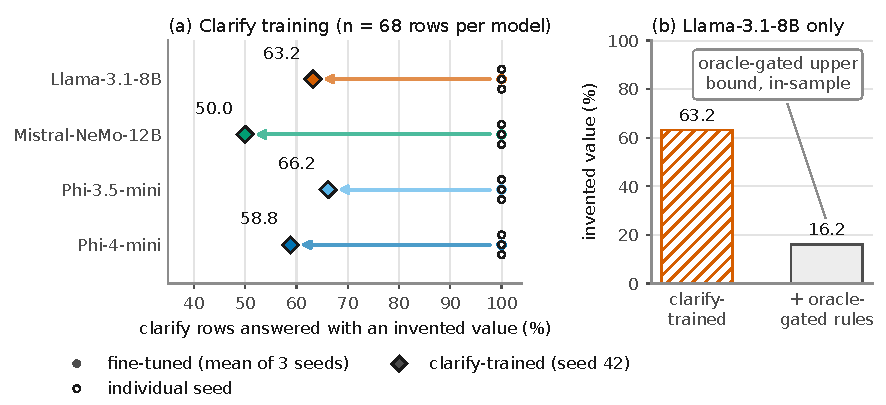
\includegraphics[width=\textwidth]{f09_mitigation}
  \caption{(a)~Invented-value rate on \TestClarify rows: fine-tuned (circles; three seeds) against clarify-trained (diamonds, seed 42). (b)~Llama-3.1-8B only: invented values remaining after clarify training, and after an oracle-gated rule set is applied to those outputs. The second bar is an in-sample upper bound, not a performance estimate; the detector reads gold labels.}
  \label{fig:mitigation}
\end{figure}

Family A5, the detector, is descriptive. Applied to clarify-trained Llama, it raises safe handling of incomplete questions from \DetLearnedPct\% to \DetCombinedPct\% (risk difference \SigAFiveDetectorDiff [\SigAFiveDetectorDiffLo, \SigAFiveDetectorDiffHi] percentage points; 32 rows caught, 0 reversed). The detector runs only on rows whose gold type is clarify, flags any invented numeric answer on the three scorable clarify categories, and had its missing-$\mathrm{ET}_0$ keywords added after the test rows were inspected. All three properties use information a deployed system would not have. The figure is an oracle-gated upper bound on what these surface rules catch in this test set. The rules are listed in \cref{app:detector}.

\section{Bengali versus English}
\label{sec:res-language}

H2 said that Bengali trails English after fine-tuning. \Cref{tab:language} and \cref{fig:language} split that claim by question type.

On factual chrF++, English is ahead in every model at seed 42 (mean differences \SigASixFacLlamaDiff to \SigASixFacPhiFourDiff points). The registered Wilcoxon test is significant after Holm in \SigASixFacSigSeedA of four models (Mistral, Phi-3.5, Phi-4) and robust on all three seeds in \RobustASixFacYes of four (the two Phi models). Llama's rank test is not significant ($p_\mathrm{Holm}$ \SigASixFacLlamaPholm; rank-biserial $r = \SigASixFacLlamaEff$ [\SigASixFacLlamaEffLo, \SigASixFacLlamaEffHi]), while the bootstrap interval of the \emph{mean} difference, \SigASixFacLlamaDiff [\SigASixFacLlamaDiffLo, \SigASixFacLlamaDiffHi] chrF++ points, excludes zero. The paired differences are skewed: a few English rows gain a lot. The registered verdict stands: no significant difference detected for Llama. Mistral's gap is significant at seed 42 only.

On numeric accuracy the picture is different. No unpaired Fisher test on the 73 versus 73 rows is significant at any seed. The confidence intervals of the English-minus-Bengali difference have half-widths of about 15 percentage points; they are too wide to rule out a gap of that size in either direction. There is no consistent sign.

% AUTO-GENERATED by scripts/thesis/tables.py
\begin{table}[tbp]
\centering
\scriptsize
\caption{Bengali versus English, fine-tuned models, seed 42 (test family A6). Numeric: share of the \NumericAll{} numeric rows correct within $\pm$0.1 mm, half in each language, compared with an unpaired Fisher exact test. Factual: chrF++ on facts asked in both languages, compared with a Wilcoxon signed-rank test; the difference is in chrF++ points. CIs are \PlanBootstrap{}-resample bootstrap intervals. ``All seeds'' says whether the factual difference is significant after Holm correction at seeds 42, 1337 and 2024.}
\label{tab:language}
\begin{tabular}{lrrlrrrlrl}
\toprule
& \multicolumn{4}{c}{Numeric, $\pm$0.1 mm (\%), \SigASixNumLlamaN{} rows} & \multicolumn{5}{c}{Factual chrF++, \SigASixFacLlamaN{} paired facts} \\
\cmidrule(lr){2-5}\cmidrule(lr){6-10}
Model & bn & en & en $-$ bn [95\% CI] & $p_\text{Holm}$ & bn & en & en $-$ bn [95\% CI] & $p_\text{Holm}$ & all seeds \\
\midrule
Llama-3.1-8B & \SigASixNumLlamaRateA{} & \SigASixNumLlamaRateB{} & \SigASixNumLlamaDiff{} [\SigASixNumLlamaDiffLo{}, \SigASixNumLlamaDiffHi{}] & \SigASixNumLlamaPholm{} & \SigASixFacLlamaRateA{} & \SigASixFacLlamaRateB{} & \SigASixFacLlamaDiff{} [\SigASixFacLlamaDiffLo{}, \SigASixFacLlamaDiffHi{}] & \SigASixFacLlamaPholm{} & \RobustASixFacLlama{} \\
Mistral-NeMo-12B & \SigASixNumMistralRateA{} & \SigASixNumMistralRateB{} & \SigASixNumMistralDiff{} [\SigASixNumMistralDiffLo{}, \SigASixNumMistralDiffHi{}] & \SigASixNumMistralPholm{} & \SigASixFacMistralRateA{} & \SigASixFacMistralRateB{} & \SigASixFacMistralDiff{} [\SigASixFacMistralDiffLo{}, \SigASixFacMistralDiffHi{}] & \SigASixFacMistralPholm{} & \RobustASixFacMistral{} \\
Phi-3.5-mini & \SigASixNumPhiThreeRateA{} & \SigASixNumPhiThreeRateB{} & \SigASixNumPhiThreeDiff{} [\SigASixNumPhiThreeDiffLo{}, \SigASixNumPhiThreeDiffHi{}] & \SigASixNumPhiThreePholm{} & \SigASixFacPhiThreeRateA{} & \SigASixFacPhiThreeRateB{} & \SigASixFacPhiThreeDiff{} [\SigASixFacPhiThreeDiffLo{}, \SigASixFacPhiThreeDiffHi{}] & \SigASixFacPhiThreePholm{} & \RobustASixFacPhiThree{} \\
Phi-4-mini & \SigASixNumPhiFourRateA{} & \SigASixNumPhiFourRateB{} & \SigASixNumPhiFourDiff{} [\SigASixNumPhiFourDiffLo{}, \SigASixNumPhiFourDiffHi{}] & \SigASixNumPhiFourPholm{} & \SigASixFacPhiFourRateA{} & \SigASixFacPhiFourRateB{} & \SigASixFacPhiFourDiff{} [\SigASixFacPhiFourDiffLo{}, \SigASixFacPhiFourDiffHi{}] & \SigASixFacPhiFourPholm{} & \RobustASixFacPhiFour{} \\
\bottomrule
\end{tabular}
\end{table}


\begin{figure}[tbp]
  \centering
  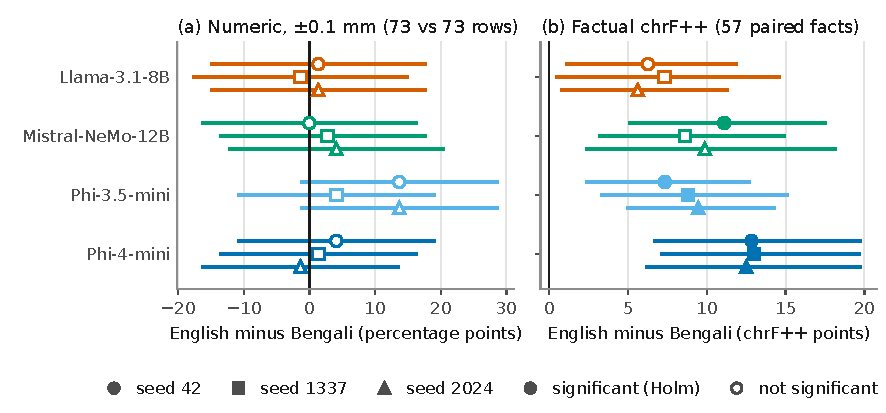
\includegraphics[width=\textwidth]{f11_language}
  \caption{English minus Bengali, fine-tuned arms, three seeds. (a)~Numeric accuracy within $\pm$0.1\,mm, 73 rows per language, unpaired. (b)~Factual chrF++, 57 paired facts. Filled markers are significant after Holm; open markers are not. Most numeric intervals include zero. The factual gap favours English and is significant at seed 42 in three of four models.}
  \label{fig:language}
\end{figure}

Human language contrasts (family B5, 100 pairs) go the same way: none of eight tests is significant after Holm. Point estimates lean English in the three fine-tuned arms. H2 is therefore only partially supported: a factual English lead that is not universal, a numeric comparison that cannot rule out a moderate gap, and no significant human difference detected.

An exploratory check, added after Part A, classifies the language of the response by script (\cref{fig:response-lang}). Zero-shot Mistral-NeMo answered only \LangMistralZSAll\% [\LangMistralZSAllLo, \LangMistralZSAllHi] of Bengali questions in Bengali, and \LangMistralZSClarify\% of Bengali clarify questions. Every fine-tuned and clarify-trained arm answered at least \RangeLangTunedMin\% in Bengali. Fine-tuning fixes response language. It also qualifies Mistral's zero-shot confident-error rate: that baseline is measured largely on English answers to Bengali questions.

\begin{figure}[tbp]
  \centering
  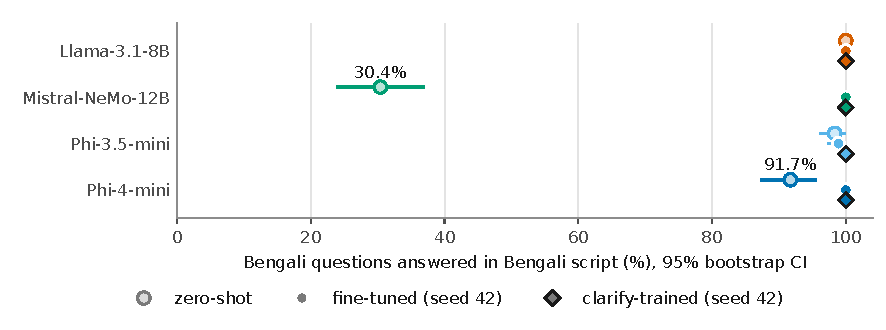
\includegraphics[width=\textwidth]{f18_response_language}
  \caption{Share of Bengali test questions answered in Bengali script (exploratory; \LangMistralZSAllN questions per arm). Open circles are zero-shot, filled circles fine-tuned (seed 42), diamonds clarify-trained. Mistral zero-shot is the only arm that routinely answers Bengali questions in English; after fine-tuning every arm is at or above \RangeLangTunedMin\%.}
  \label{fig:response-lang}
\end{figure}

\section{Human Evaluation}
\label{sec:res-human}

H3 named two primary agreement measures before testing, with a threshold of \AgreeThreshold: Fleiss' $\kappa$ on the farmer decision and ordinal Krippendorff's $\alpha$ on the 1--5 rating. \Cref{tab:agreement} reports both, with bootstrap intervals over the \HumOverlapOutputs shared outputs. Farmer $\kappa$ is \AgrKappaFarmer [\AgrKappaFarmerLo, \AgrKappaFarmerHi]; ordinal $\alpha$ is \AgrAlphaOrdinal [\AgrAlphaOrdinalLo, \AgrAlphaOrdinalHi]. Both clear the threshold. Nominal $\kappa$ on the raw 1--5 scale is \AgrKappaNominal [\AgrKappaNominalLo, \AgrKappaNominalHi]; it treats a 4-versus-5 disagreement as a full disagreement and so understates agreement on an ordinal scale. It is reported for completeness, not as a primary measure. H3 is supported on the pre-specified primary measures.

Leave-one-out ordinal $\alpha$ rises to \AgreeAlphaWithoutOneRecomputed without annotator A1 and falls without any of the others (\cref{fig:annotators}). Sensitivity analyses that drop A1, and that add the \HumAuthored authored translations, change no human verdict (\cref{sec:impl-plan}).

% AUTO-GENERATED by scripts/thesis/tables.py
\begin{table}[tbp]
\centering
\footnotesize
\caption{Agreement on the \HumOverlapOutputs{} outputs rated by all five annotators, with 95\% bootstrap CIs over items. The two primary measures were named before significance testing. Nominal $\kappa$ treats adjacent ratings (four versus five) as full disagreement and so understates agreement on an ordinal scale; it is reported for completeness. Leave-one-out values were recomputed and reproduce the audit report's all-annotator and without-A1 values.}
\label{tab:agreement}
\begin{tabular}{llrl}
\toprule
Measure & Statistic & Value & 95\% CI \\
\midrule
Would give to a farmer & Fleiss' $\kappa$ (primary) & \AgrKappaFarmer{} & [\AgrKappaFarmerLo{}, \AgrKappaFarmerHi{}] \\
Would give to a farmer & Krippendorff's $\alpha$, nominal & \AgrAlphaFarmer{} & [\AgrAlphaFarmerLo{}, \AgrAlphaFarmerHi{}] \\
Rating 1--5 & Krippendorff's $\alpha$, ordinal (primary) & \AgrAlphaOrdinal{} & [\AgrAlphaOrdinalLo{}, \AgrAlphaOrdinalHi{}] \\
Rating 1--5 & Krippendorff's $\alpha$, interval & \AgrAlphaInterval{} & [\AgrAlphaIntervalLo{}, \AgrAlphaIntervalHi{}] \\
Rating, three bands & Fleiss' $\kappa$ & \AgrKappaBands{} & [\AgrKappaBandsLo{}, \AgrKappaBandsHi{}] \\
Rating 1--5 & Fleiss' $\kappa$, nominal & \AgrKappaNominal{} & [\AgrKappaNominalLo{}, \AgrKappaNominalHi{}] \\
\addlinespace
Rating, leave one out & ordinal $\alpha$ without A1 / A2 / A3 / A4 / A5 & \multicolumn{2}{l}{\AgreeAlphaWithoutOneRecomputed{} / \AgreeAlphaWithoutTwoRecomputed{} / \AgreeAlphaWithoutThreeRecomputed{} / \AgreeAlphaWithoutFourRecomputed{} / \AgreeAlphaWithoutFiveRecomputed{}} \\
\bottomrule
\end{tabular}
\end{table}


\begin{figure}[tbp]
  \centering
  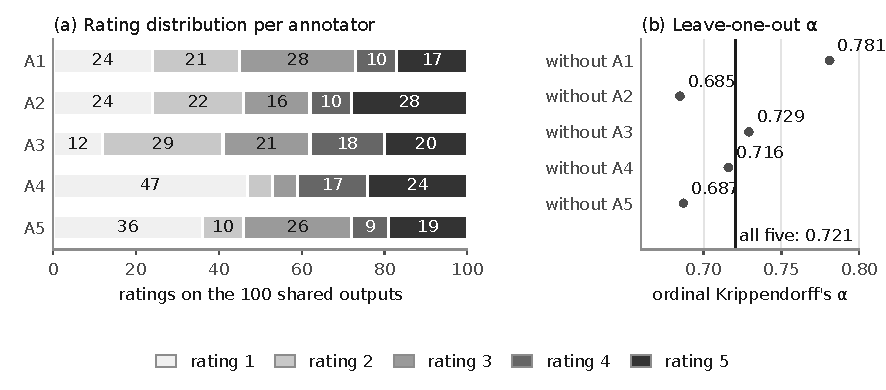
\includegraphics[width=\textwidth]{f14_annotators}
  \caption{(a)~Rating distribution of each annotator on the \HumOverlapOutputs shared outputs. (b)~Ordinal $\alpha$ when that annotator is left out; the vertical line is $\alpha$ with all five. Leaving out A1 raises agreement; leaving out any other annotator lowers it.}
  \label{fig:annotators}
\end{figure}

\Cref{tab:human-results} and \cref{fig:human-qtype} are the arm-level human scores on the primary sample. Fine-tuning raises mean rating from \HumTestZSRating [\HumTestZSRatingLo, \HumTestZSRatingHi] to \HumTestFTRating [\HumTestFTRatingLo, \HumTestFTRatingHi] and farmer-yes from \HumTestZSYes [\HumTestZSYesLo, \HumTestZSYesHi]\% to \HumTestFTYes [\HumTestFTYesLo, \HumTestFTYesHi]\% (B2-i and B3-i; both $p_\mathrm{Holm}$ below .001). That corroborates H1. On clarify questions the standard fine-tuned arms are judged unfit to give a farmer on every primary-sample item (\HumTestFTClarifyYes\% for Llama FT; the Mistral cell is the same 0 of \HumTestFTClarifyN). The clarify-trained arm reaches \HumTestCLClarifyYes\% [\HumTestCLClarifyYesLo, \HumTestCLClarifyYesHi] farmer-yes on those questions (B3-ii clarify: $+$\,\SigBThreeClVsFtClarifyDiff [\SigBThreeClVsFtClarifyDiffLo, \SigBThreeClVsFtClarifyDiffHi] percentage points, $p_\mathrm{Holm}$ below .001), which corroborates C1.

The overall clarify-versus-fine-tuned contrast is measure-dependent. Farmer-yes rises by \SigBThreeClVsFtOverallDiff [\SigBThreeClVsFtOverallDiffLo, \SigBThreeClVsFtOverallDiffHi] percentage points and survives Holm ($p_\mathrm{Holm}$ \SigBThreeClVsFtOverallPholm). Mean rating rises by less and does not ($p_\mathrm{Holm}$ \SigBTwoClVsFtOverallPholm). The annotator-adjusted model finds the rating contrast significant when it is not corrected for multiplicity; B2's corrected verdict stands. Report the overall human benefit of clarify training as significant on farmer-yes and not on rating after correction.

% AUTO-GENERATED by scripts/thesis/tables.py
\begin{table}[tbp]
\centering
\scriptsize
\caption{Human results per arm on the primary sample of \HumTestFTN{} test-set questions, with 95\% bootstrap CIs. A shared output's score is the mean of its five ratings and its farmer decision is the majority vote. ``Acceptable'' means a mean rating of at least four. The clarify column covers the \HumTestFTClarifyN{} clarify questions in the primary sample. The last column adds the \HumAuthored{} authored Bengali translations (sensitivity sample). Raw means do not adjust for which annotator rated which output; the annotator-adjusted models (B4) leave every contrast's direction and significance unchanged.}
\label{tab:human-results}
\begin{tabular}{lllllr}
\toprule
Arm & Mean rating (1--5) & Farmer yes (\%) & Acceptable (\%) & Clarify yes (\%) & All \HumQuestions{}: yes (\%) \\
\midrule
Llama zero-shot & \HumTestZSRating{} [\HumTestZSRatingLo{}, \HumTestZSRatingHi{}] & \HumTestZSYes{} [\HumTestZSYesLo{}, \HumTestZSYesHi{}] & \HumTestZSGood{} [\HumTestZSGoodLo{}, \HumTestZSGoodHi{}] & \HumTestZSClarifyYes{} & \HumAllZSYes{} \\
Llama fine-tuned & \HumTestFTRating{} [\HumTestFTRatingLo{}, \HumTestFTRatingHi{}] & \HumTestFTYes{} [\HumTestFTYesLo{}, \HumTestFTYesHi{}] & \HumTestFTGood{} [\HumTestFTGoodLo{}, \HumTestFTGoodHi{}] & \HumTestFTClarifyYes{} & \HumAllFTYes{} \\
Llama clarify-trained & \HumTestCLRating{} [\HumTestCLRatingLo{}, \HumTestCLRatingHi{}] & \HumTestCLYes{} [\HumTestCLYesLo{}, \HumTestCLYesHi{}] & \HumTestCLGood{} [\HumTestCLGoodLo{}, \HumTestCLGoodHi{}] & \HumTestCLClarifyYes{} & \HumAllCLYes{} \\
Mistral fine-tuned & \HumTestMisRating{} [\HumTestMisRatingLo{}, \HumTestMisRatingHi{}] & \HumTestMisYes{} [\HumTestMisYesLo{}, \HumTestMisYesHi{}] & \HumTestMisGood{} [\HumTestMisGoodLo{}, \HumTestMisGoodHi{}] & \HumTestMisClarifyYes{} & \HumAllMisYes{} \\
\bottomrule
\end{tabular}
\end{table}


\begin{figure}[tbp]
  \centering
  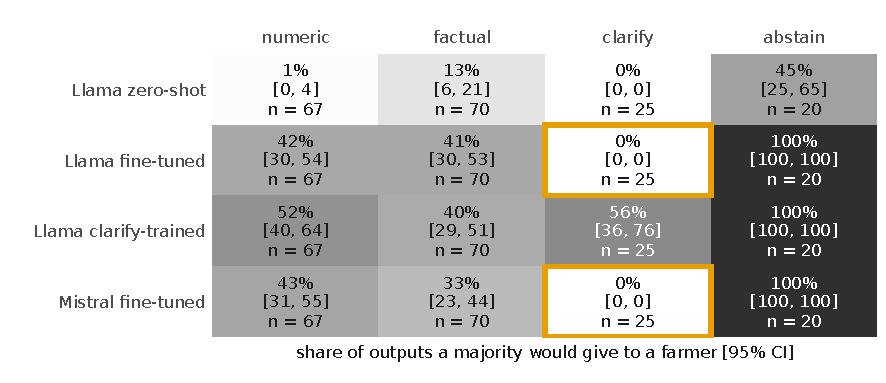
\includegraphics[width=\textwidth]{f12_human_by_qtype}
  \caption{Share of outputs a majority would give to a farmer, by arm and question type, primary sample, with 95\% CIs. The highlighted cells are incomplete questions: 0\% for both standard fine-tuned arms, \HumTestCLClarifyYes\% for Llama clarify-trained.}
  \label{fig:human-qtype}
\end{figure}

Human acceptance of numeric answers tracks agreement with the visible reference, not the $\pm$0.1\,mm headline. Spearman $\rho$ between absolute error and mean rating is \SigBEightRhoEff [\SigBEightRhoEffLo, \SigBEightRhoEffHi] on \SigBEightRhoN fine-tuned numeric outputs ($p_\mathrm{Holm}$ below .001; 21 multi-crop outputs have no scalar error and are dropped). \Cref{fig:acceptance} bins the same outputs. Annotators accepted \BinBExactYes\% of exact matches (below 0.005\,mm) and \BinBPtOneYes\% of answers 0.005--0.1\,mm away; the 0.1--1.0\,mm bin is accepted \BinBOneYes\% of the time. The registered headline, that acceptance tracks $\pm$0.1\,mm rather than $\pm$1\,mm, holds. The additional finding is that $\pm$0.1\,mm is more lenient than the human standard: \texttt{exact\_0.1} counts as correct many answers raters would not hand over.

\begin{figure}[tbp]
  \centering
  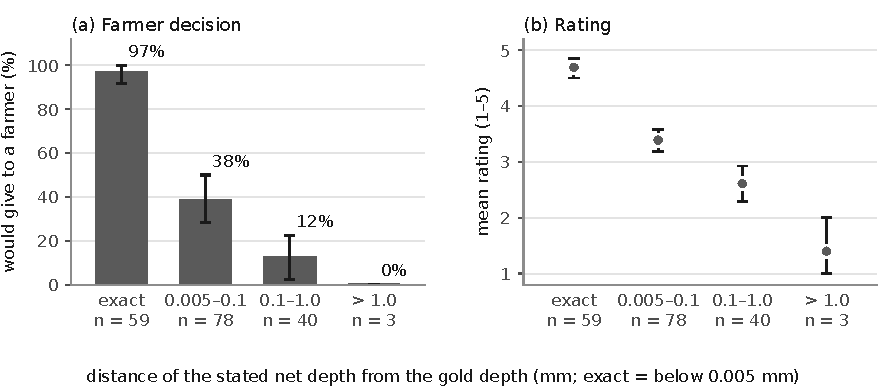
\includegraphics[width=\textwidth]{f17_acceptance_by_distance}
  \caption{Human acceptance (a) and mean rating (b) by distance of the stated net depth from the gold, three fine-tuned arms, primary numeric questions. With the reference visible, raters accepted \BinBExactYes\% of exact answers and \BinBPtOneYes\% of answers inside the 0.005--0.1\,mm band that the automatic headline still counts as correct.}
  \label{fig:acceptance}
\end{figure}

Word-level Dice is the automatic factual metric that best tracks the farmer decision (ROC-AUC \ValDiceWordAuc [\ValDiceWordAucLo, \ValDiceWordAucHi] on 280 factual judgements). Its interval overlaps ROUGE-L and chrF++. Character-level Dice tracks worst. That closes the deferred metric check: chrF++ remains the headline because it was fixed before results, and Dice is the closest of the set to the raters.

\section{Llama Fine-Tuned versus Mistral Fine-Tuned}
\label{sec:res-models}

The pre-registered comparison of the two large models after fine-tuning found no significant difference. On numeric \texttt{correct\_0p1}, Mistral minus Llama is \SigATwoLlamaVsMistralDiff [\SigATwoLlamaVsMistralDiffLo, \SigATwoLlamaVsMistralDiffHi] percentage points (McNemar odds ratio \SigATwoLlamaVsMistralEff [\SigATwoLlamaVsMistralEffLo, \SigATwoLlamaVsMistralEffHi]), non-significant at all three seeds. Human rating and farmer-yes go the same way (B2-iii, B3-iii), and the annotator-adjusted models leave direction and significance unchanged. The four fine-tuned models do differ as a set (Friedman $W = \SigATwoFriedmanEff$ [\SigATwoFriedmanEffLo, \SigATwoFriedmanEffHi]); the pre-specified tier contrast, \{Llama, Mistral\} minus \{Phi-3.5, Phi-4\}, is significant and robust. \Cref{fig:forest} places these effects next to the others.

\begin{figure}[tbp]
  \centering
  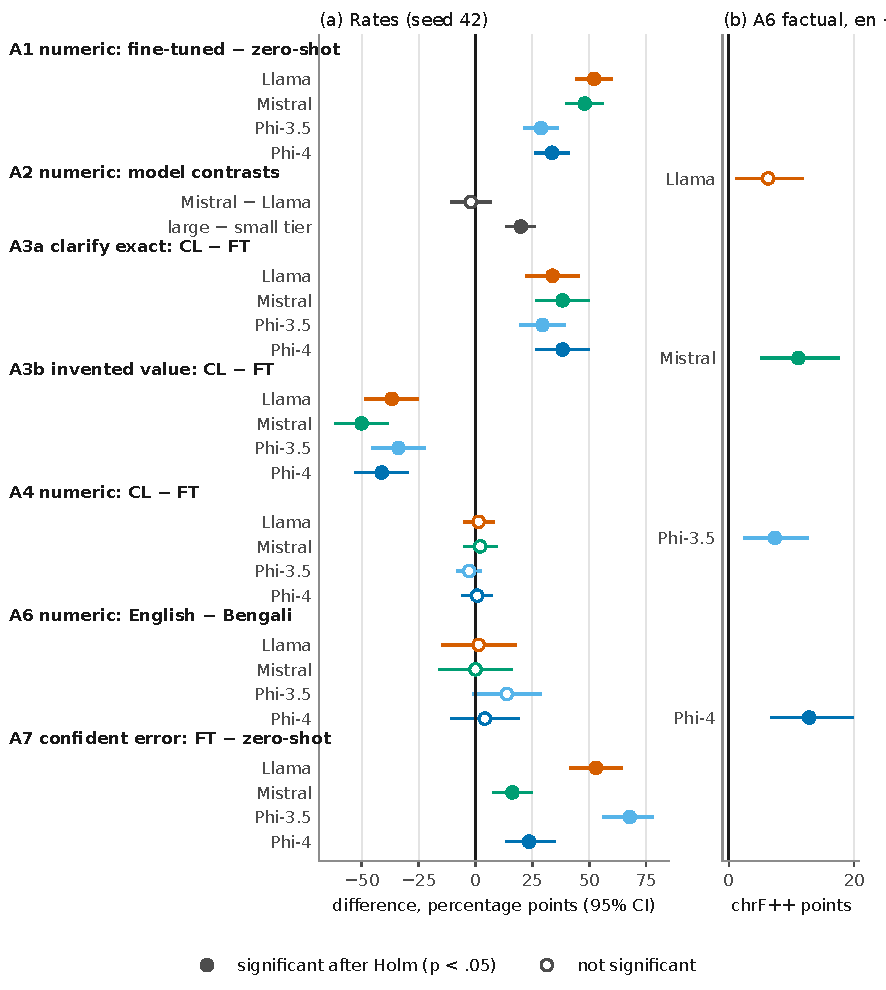
\includegraphics[width=\textwidth]{f16_forest}
  \caption{Primary automatic effects at seed 42 with 95\% CIs. (a)~Rate differences in percentage points. (b)~Factual English-minus-Bengali chrF++. Filled markers are significant after Holm. A1, A3, A7 and the tier contrast sit away from zero; A2 (Mistral minus Llama), A4 (clarify-trained minus fine-tuned numeric) and A6 numeric include zero.}
  \label{fig:forest}
\end{figure}

\section{Hypothesis Summary}
\label{sec:res-summary}

% AUTO-GENERATED by scripts/thesis/tables.py
\begin{table}[tbp]
\centering
\scriptsize
\caption{Hypothesis verdicts under the analysis plan fixed before significance testing (plan v3). Automatic tests use seed 42 with Holm correction within each family; human tests use the primary sample of \HumInTest{} test-set questions. pp = percentage points; intervals are 95\% bootstrap CIs.}
\label{tab:verdicts}
\begin{tabular}{l>{\raggedright\arraybackslash}p{0.2\textwidth}>{\raggedright\arraybackslash}p{0.12\textwidth}>{\raggedright\arraybackslash}p{0.2\textwidth}>{\raggedright\arraybackslash}p{0.3\textwidth}}
\toprule
ID & Claim & Tests & Verdict & Key numbers \\
\midrule
H1 & Fine-tuning beats zero-shot & A1, B2-i, B3-i & Supported; robust on all three seeds & A1: \RangeSigAOneDiffMin{} to \RangeSigAOneDiffMax{} pp, every $p_\text{Holm}$ \SigAOneLlamaPholm{}; farmer yes \SigBThreeFtVsZsOverallDiff{} [\SigBThreeFtVsZsOverallDiffLo{}, \SigBThreeFtVsZsOverallDiffHi{}] pp \\
H2 & Bengali trails English & A6, B5 & Partially supported & factual: significant in \SigASixFacSigSeedA{} of four models at seed 42, \RobustASixFacYes{} of four on all seeds; numeric: \SigASixNumSigAnySeed{} of \SigASixNumTestsAllSeeds{} tests; human: \SigBFiveSig{} of \SigBFiveTests{} \\
H3 & Annotators agree & B6 & Supported on the primary measures & farmer $\kappa$ \AgrKappaFarmer{} [\AgrKappaFarmerLo{}, \AgrKappaFarmerHi{}]; ordinal $\alpha$ \AgrAlphaOrdinal{} [\AgrAlphaOrdinalLo{}, \AgrAlphaOrdinalHi{}] \\
T & Fine-tuning turns invented values into confident errors & A7 & Supported in all four models on all seeds; size depends on the base model & \RangeSigASevenDiffMin{} to \RangeSigASevenDiffMax{} pp; fine-tuned strict rate \RangeFTSeedAConfErrBMin{}--\RangeFTSeedAConfErrBMax{}\% \\
C1 & Clarify training teaches clarification & A3a, B3-ii & Supported & +\RangeSigAThreeADiffMin{} to +\RangeSigAThreeADiffMax{} pp; human clarify cell \SigBThreeClVsFtClarifyDiff{} [\SigBThreeClVsFtClarifyDiffLo{}, \SigBThreeClVsFtClarifyDiffHi{}] pp \\
C2 & Clarify training reduces invented values & A3b & Supported & $-$\RangeSigAThreeBDiffMin{} to $-$\RangeSigAThreeBDiffMax{} pp \\
C3 & Clarify training does not harm numeric accuracy & A4 & No loss detected & \SigAFourSig{} of four significant; lowest CI bound \SigAFourWorstLo{} pp \\
D & A detector adds safety & A5 & Descriptive only: oracle-gated upper bound & \SigAFiveDetectorDiff{} [\SigAFiveDetectorDiffLo{}, \SigAFiveDetectorDiffHi{}] pp, no test \\
M & Llama FT differs from Mistral FT & A2, B2-iii, B3-iii, B4 & No significant difference detected & \SigATwoLlamaVsMistralDiff{} [\SigATwoLlamaVsMistralDiffLo{}, \SigATwoLlamaVsMistralDiffHi{}] pp; farmer yes \SigBThreeMisVsFtOverallDiff{} [\SigBThreeMisVsFtOverallDiffLo{}, \SigBThreeMisVsFtOverallDiffHi{}] pp \\
\bottomrule
\end{tabular}
\end{table}


\Cref{tab:verdicts} is the register of verdicts. Nothing in it reversed a pre-specified direction. Three Stage 6 readings were qualified once tested: the factual English lead is not universal; $\pm$0.1\,mm is more lenient than human acceptance; and the detector figure is not a performance estimate. Clarify training's overall human benefit is significant on farmer-yes and not on rating after Holm. Mistral zero-shot answered most Bengali questions in English, which the Stage 6 metrics did not distinguish from Bengali answers.

\section{Threats to Validity}
\label{sec:threats}

\paragraph{Construct.}
The confident-error definition depends on a response classifier, a parser and a re-tokenised length. Decode-then-encode is not perfectly idempotent; the threshold was kept as registered and the bias is conservative for T. The Bengali hedge list under-detects zero-shot hedging and does not affect any fine-tuned row we checked. Numeric ``accuracy'' is agreement with this system's calculator, including its unclamped zero depths and its project-specific rainfall rule. Human ratings were made with the gold visible and with a rubric that tells raters to score invented values 1, so they corroborate the automatic measures rather than independently testing field usefulness. Annotators are not agricultural experts.

\paragraph{Internal.}
The twelve fine-tuned runs share data and base weights; seeds measure training randomness, not independent samples. Clarify-trained arms exist at one seed, so C1--C3 cannot be called robust. Three metric definitions were changed after results were seen; each was checked against a gold-oracle arm whose score after the changes is \ChangeOracleAfter, and whose score before them is not in any surviving file. The analysis plan was fixed before significance tests and after the descriptive results; we do not call it pre-registered. A5 reads gold labels. The semantic leakage review is still pending (\PENDINGREVIEW{semantic leakage review, \LeakReviewSample pairs}). Digitisation of the calendars has not been independently checked (\STAGEEIGHTB{digitisation check}).

\paragraph{External.}
All questions are synthetic. No farmer took part. Four open-weight models, none larger than 12B, and no commercial model. Abstention is measured on easy seed out-of-domain rows; \TestExcluded adversarial rows are unscored. There is no system prompt and no calculator in the loop, so the study measures what fine-tuning does on its own, not what an instructed or tool-using system would do. The prompted baseline is \STAGEEIGHTB{prompted baseline}. Retrieval was not compared. Results are for this coefficient table, this rainfall rule and this template style.

\paragraph{Statistical.}
Holm correction is within family, not across the whole plan. Numeric language tests are unpaired and underpowered; their intervals do not rule out gaps of about 15 percentage points. MixedLM treats the rating as interval; the Bayesian farmer-yes model yields credible intervals, not $p$-values. We never read a non-significant test as equivalence.
